\chapter{Project realization}
\section*{Introduction}
This chapter covers the implementation, testing and the deployment processes of
the Benchmarks dashboard project. To deal wit each of these processes, we will
introduce the technologies used and describe the way we used them. In
addition, we will present the project planning.
\pagebreak

\section{Used technologies}
\subsection{Programming languages}
\subsubsection{Python}
Python is an interpreted, interactive, object-oriented programming language. It
incorporates modules, exceptions, dynamic typing, very high level dynamic data
types, and classes. Python combines remarkable power with very clear syntax. It
has interfaces to many system calls and libraries, as well as to various window
systems, and is extensible in C or C++. It is also usable as an extension
language for applications that need a programmable interface. Finally, Python is
portable: it runs on many Unix variants, on the Mac, and on PCs under MS-DOS,
Windows, Windows NT, and OS/2.

Python is a high-level general-purpose programming language that can be applied
to many different classes of problems. The language comes with a large standard
library that covers areas such as string processing (regular expressions,
Unicode, calculating differences between files), Internet protocols (HTTP, FTP,
SMTP, XML-RPC, POP, IMAP, CGI programming), software engineering (unit testing,
logging, profiling, parsing Python code), and operating system interfaces
(system calls, filesystem, TCP/IP sockets). Look at the table of contents for
The Python Standard Library to get an idea of what's available. A wide variety
of third-party extensions are also available.\cite{python}


\subsubsection{Javascript}
JavaScript (shortened to JS) is an interpreted, object-oriented, weakly typed,
programming language with first-class functions most known as scripting language
for Web pages. It was originally implemented so that client-side scripts could
interact with the user, control the browser, communicate asynchronously and
alter the web page content that was displayed, and now it has evaluated to
involve game  development and applications creation. JavaScript's main purpose
was the creation and embedding of scripts in the HTML client side in order to
guarantee more interactivity with the user. It was created to offer dynamic
tasks such as the transformation of the page elements, visual effects and
immediate reactions to the user actions. But now JS for server-side web is
gaining popularity with the appearance of JavaScript frameworks for that
purpose. 
JavaScript was a purely interpreted language. This means that scripts execute
without preliminary compilation (without conversion of the script text into
machine code). The user's browser interprets the script, that is, analyzes and
immediately executes it. In modern implemented, The user's browser interprets
the script, that is, analyzes and immediately. \cite{javascript}

\subsection{Frameworks}
\subsubsection{Pyramid}
Pyramid is a fast and low-level Python web framework. It is developed as
part of the Pylons Projects. Even Pyramid isn't famous like Flask and Django, it
minimal, unobtrusive and agnostic design helps in developing more robust and
fast web applications.

\subsubsection{ReactJS}
React is an open-source front end library developed by Facebook. It's used for
handling view layer for web and mobile apps. ReactJS allows us to create large
web applications that use data which can change over time, without reloading the
page, using reusable UI components. Its main goal is to be fast, simple and
scalable. It is currently one of the most popular JavaScript libraries and it
has strong foundation and large community behind it. React components are
typically written in JSX, a JavaScript extension syntax allowing quoting of HTML
and using HTML tag syntax to render sub-components.

\subsubsection{Grommet}
Grommet \cite{grommet} is a UX framework for enterprise applications developed by HP, on top of
ReactJS. It was created to align the design and developer workflow into one
seamless experience. The Grommet components \cite{grommet_comp} library is designed to be perfect
complement to the design system. With little setup, developer will be able to
create a Grommet application from scratch in minutes and take the pain out of
translating design files into running application code.

\subsection{Tools and services}
\subsubsection{AWS}
Amazon Web Services (AWS) is a subsidiary of Amazon.com that provides on-demand
cloud computing platforms. These services operate from many global geographical
regions including 6 in North America. They include Amazon Elastic Compute
Cloud, also known as "EC2", and Amazon Simple Storage Service, also known as
"S3". As of 2016, AWS has more than 70 services, spanning a wide range,
including compute, storage, networking, database, analytics, application
services, deployment, management, mobile, developer tools and tools for the
Internet of Things. Amazon markets AWS as a service to provide large computing
capacity quicker and cheaper than a client company building an actual physical
server farm.

\subsubsection{Nix}

Nix \cite{nix_elphd} is a purely functional package manager. This means that it treats packages
like values in purely functional programming languages such as Haskell — they
are built by functions that don’t have side-effects, and they never change after
they have been built. Nix stores packages in the Nix store, usually the
directory /nix/store, where each package has its own unique sub-directory such as

\colorbox{Gray}{\lstinline{nix/store/b6gvzjyb2pg0kjfwrjmg1vfhh54ad73z-firefox-33.1/}}

Where \colorbox{Gray}{\lstinline{b6gvzjyb2pg0...}} is a unique identifier for the package that captures all its
dependencies (it’s a cryptographic hash of the package’s build dependency
graph). This enables many powerful features.

Nix was created by Eelco Dolstra as PhD project. Eelco is, along with other main
contributors to the Nix ecosystem, employed as DevOps engineer at Predictix.
\paragraph{Nix language}
The Nix expression language is a pure, lazy, functional language. Purity means
that operations in the language don't have side-effects (for instance, there is
no variable assignment). Laziness means that arguments to functions are
evaluated only when they are needed. Functional means that functions are
“normal” values that can be passed around and manipulated in interesting ways.
The language is not a full-featured, general purpose language. Its main job is
to describe packages, compositions of packages, and the variability within
packages.

\paragraph{NixOS}
Nixos is Linux distribution built on top of the Nix package manager. It
uses the Nix language for declarative configuration which allows reliable
system upgrades.
Although NixOS started as a research project, it is a fully functional and
usable operating system.

\paragraph{NixOps}
NixOps \cite{nixops}is a tool for deploying sets of NixOS Linux Machines, either to real
hardware or to virtual machines. It extends NixOS's declarative approach to
system configuration to networks and adds provisioning.

\par
The NixOps Dashboard is a built-in house extension to NixOps and offers the same
content and functionality via a Web UI and a rich RESTful API. Core features
are:

\begin{itemize}
\item User-friendly web-based interface
\item Improved security
\item Scheduled operations (deployments, backups, ...etc)
\item Permanent traceability
\item Clear audit trail
\item Role based access
\end{itemize}

We will be using NixOps Dashboard API to provision servers and deploy the
applications in the cloud in order to benchmark them in a production-like
systems.

\section{Development environment}
Below are the characteristics of the development machine we used during the
project implementation.

\begin{itemize}
  \item{\textbf{Processor}: Intel® Core™ i7-3540M CP}
  \item{\textbf{RAM}: 16 GO DDR3 }
  \item{\textbf{System}: Ubuntu Linux 14.04 LTS}
\end{itemize}


\section{Project management}
This section gives an overview of the project management process of the
Benchmarks Dashboard application. At first, we will start by introducing the
project team and then we will describe the tracking process of the different
implementation tasks.
\subsection{Project team}
The table \hyperref[project_members]{\ref{project_member}} introduces the project team members and their roles.

\begin{table}[]
\centering
\label{project_members}
  \begin{tabular}{ | p{3cm}  | p{6cm} |}
    \hline

    Scrum role    & Name          \\ \hline

    Product owner & Oussama Elkaceh \\ \hline
    Scrum Master  & Wassel Msehli   \\ \hline
    Team members  & Chaker Benhamed \\ \hline

    \hline
  \end{tabular}
\caption{Project members and their role}
\end{table}

\subsection{Jira}
Predictix development teams use Jira for managing the projects. Jira is a
commercial software product developed by Atlassian. It is used for bug tracking,
issue tracking and project management. Jira allow prioritizing, assigning,
tracking, reporting and auditing issues. Indeed, it improves productivity by
cutting down on time wasted on tracking issues and coordination. In fact, it
keeps the team on track and allows the project manager to monitor the progress
on projects. Besides, it improves quality be ensuring that all tasks are
recorded down with all details and followed up until accomplishment. Moreover,
Jira is an extensible platform which means that it offers workflow customization
to match more the business process. \cite{jira}


\section{Implementation}
\subsection{Achieved work}
This section is a description of the four sprints and the results we achieved at
the end of all of the sprints.
\subsection{Sprint 1}
In the first sprint, our goal is to start by automating the benchmark of one of
Predictix's applications, thus we can understand how to generalize for all other
project and solve issue of consistency. The application we worked on is THD-AP.
We started by installing the application locally understand how to build it,
This included how to compile the application, install it and run the tests.
We also deploy it in the cloud and run the benchmark tests in cloud server.
After getting acquainted to the benchmark process. We started by automating the
benchmark process by adding systemd services to Install the application, Load
the data and run the benchmarks


\subsection{Sprint 3}
In the second sprint, our goal is to model the web application that the users
will use to both start benchmarks and visualize the benchmarks runs. We stated
by looking the available frameworks for web development. Finally we developed
the workflow that will run new benchmark.

After we get acquainted to the benchmark process, we started righting defining
the steps in the benchmark pipeline.
\subsubsection{Deploying}
To be tested in production-like environment, the
application need to be deployed to the cloud. In order to compare between
benchmarks runs the server in which the application will be deployed need to be
consistent across all the runs The user mustn't have any interaction with the
provisioning of the server nor the deployment of the application. 

$\bullet$ \textbf{Provisioning}: Since Predictix application are
memory-intensive, we chose to deploy them in a r3.4xlarge EC2 instances
\cite{ec2_instances} from Amazon AWS. This type of instances offer lower price
of GiB of RAM. r3.4xlarge has 122 GB of RAM with 16 cores CPU and 320 GB of SSD
Storage.

$\bullet$ \textbf{Installing}:After provisioning the server. We need to deploy
the application to that server. The closure of the application will be already
built in Hydra. We will be using an existent nix configuration to install the
application. It uses a systemd service called \emph{install-app}. This service
will start the database, the web-server, install workspaces and it will make
sure that the application is up and running.

For starting the deployment we use NixOps Dashboard, it will take
some arguments like the type of the instance, AWS account to use to deploy
the application, The application configuration (Users, Whether to run workflows
or not...) and application closure (package). And start deploying the
application with those configurations. After NixOps finish creating the instance
in EC2 cloud. It will install the packages using predefined instructions to
install LB applications.

\subsubsection{Load data}
Loading data is project specific, each application need to provide the steps to
download data from S3, extract them and run the necessary workflows to load the
data into the database. Those steps will be written in a script called
\emph{load-perf-data.sh} by the application developers, the script will be ran as
soon as the application in installed. It will be expected to be at the script
directory within the application root directory. The figure
\hyperref[fig:load-perf-data]{\ref{fig:load-perf-data}} shows the definition of
the systemd service \emph{load-perf-data.sh}. And the figure
\hyperref[fig:load-perf-data-log]{\ref{fig:load-perf-data-log}} Shows
the log of systemd service and how the service is invoked automatically.
\begin{figure}[h]
  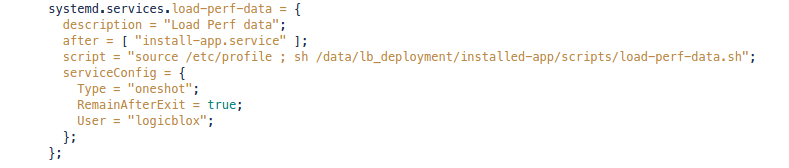
\includegraphics[width=14cm]{load-perf-data}
\caption{Load perf data nix expression}
\label{fig:load-perf-data}
\end{figure}

\begin{figure}[h]
  \centerline{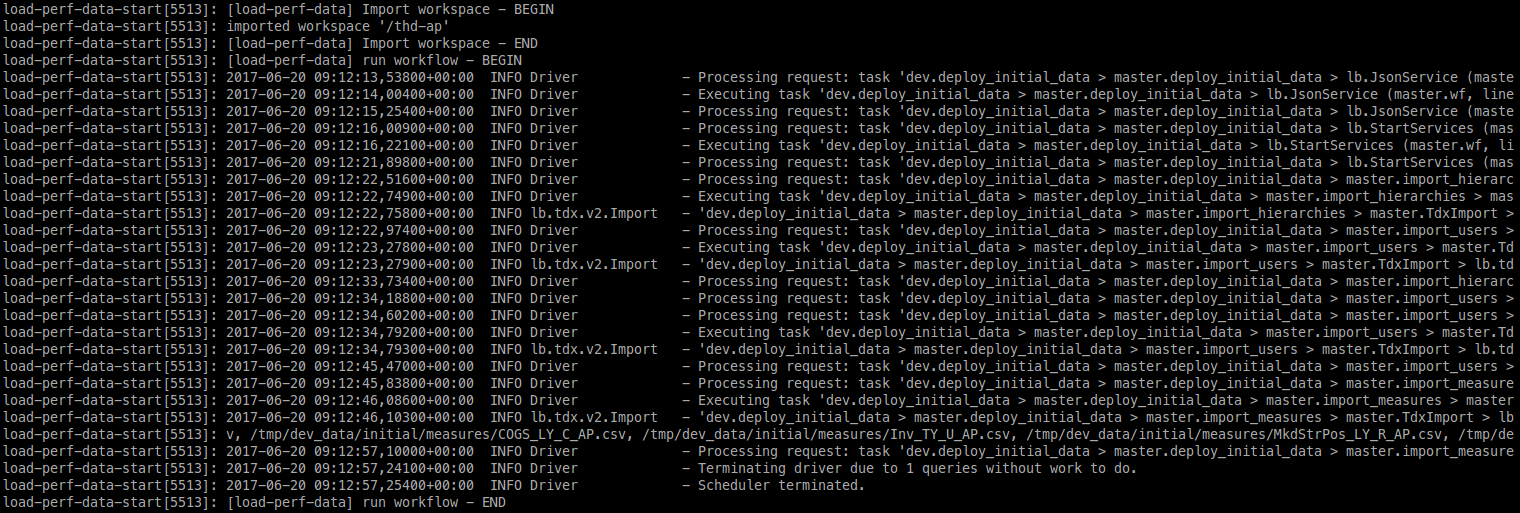
\includegraphics[width=14cm]{load-perf-data-log}}
\caption{load-perf-data log}
\label{fig:load-perf-data-log}
\end{figure}

\subsubsection{Running benchmark tests}
For running tests we use a generic script called \emph{run-perf}. This script will
define the instruction for running the tests, collect the logs, generate the
report and upload it to S3. The figure
\hyperref[fig:perf-runner-nix]{\ref{fig:perf-runner-nix}} shows the definition of
the systemd service \emph{perf-runner} responsible for running the script, it
will be launched as soon as the data is loaded with the \emph{load-perf-data}
service.
\begin{figure}[h]
  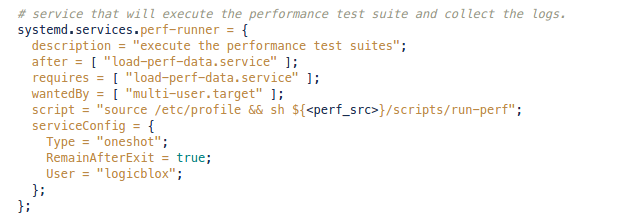
\includegraphics[width=14cm]{perf-runner-nix}
  \caption{perf-runner nix expression}
\label{fig:perf-runner-nix}
\end{figure}

\begin{figure}[h]
  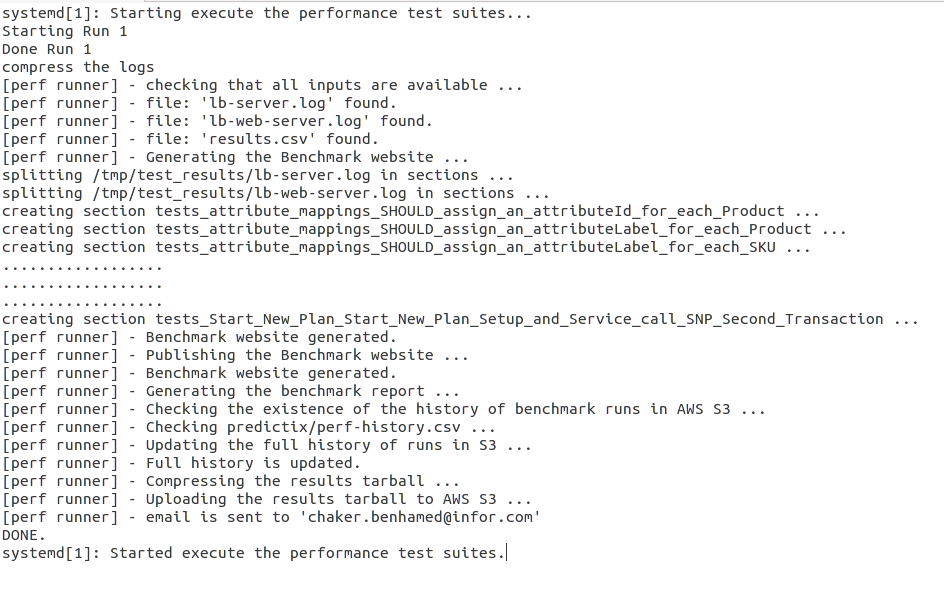
\includegraphics[width=14cm]{perf-runner-log}
  \caption{perf-runner log}
\label{fig:perf-runner-log}
\end{figure}
The figure \hyperref[fig:perf-runner-log]{\ref{fig:perf-runner-log}} shows a
truncated log of perf-runner service.

Finally after the test are completed and the report are generated they will be
automatically published to our application using the HTTP protocol.

\subsection{Sprint 3}
In the second sprint, our goal is to model the web application that the users
will use to both start benchmarks and visualize the benchmarks runs. We started
by choosing web framework.
The web ecosystem has been evolving with consistent rate over the last few
years. Having in mind that the application need to be modular, maintainable and
stable. Also from the fact that the company made a strategic decision to move to
React JS, Thus most of the frontend developers in the company are familiar with
React. We choose it to build the frontend of our application.

React helps in defining the application frontend in a declarative approach.
Component in react are like class functions in a pure functional language. The
whole and single purpose of a react component is to render an object using the
passed state. Most of the component that we wrote are stateless in the meaning
that they don't depend of the application state to render. All the data that the
component need to successfully render are passed to it in the instantiation
time. This type of component are called presentational component.

We also used the Redux library that help to organize the overall state of the
application. The later is  saved in a one big data object that called Store,
Redux then work using an action-dispatch paradigm. Component aren't responsible
of getting the data from the backend and changing the store content. If a data
need to be fetched, let's say user click on a button, then they only need to
dispatch action. When an action finish the store will be updated and redux/react
will only update the component that need to be updated. The
figure \hyperref[fig:react_redux]{\ref{fig:react_redux}} present the
difference between a react application that use redux and another one that
don't. Figure \hyperref[fig:react_workflow]{\ref{fig:react_workflow}} shows the
workflow of action dispatching in a react application.

\begin{figure}[h]
  \centerline{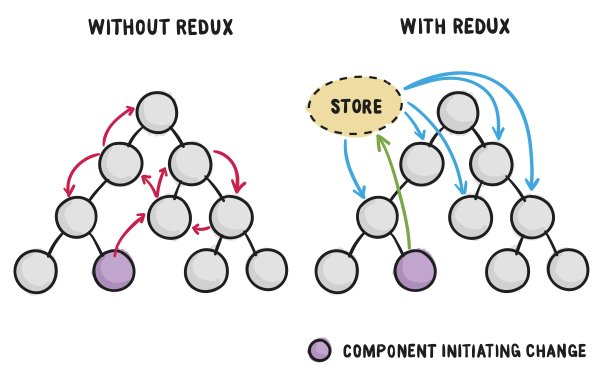
\includegraphics[width=14cm]{react_redux}}
\caption{React application with and without Redux}
\label{fig:react_redux}
\end{figure}

\begin{figure}[h]
  \centerline{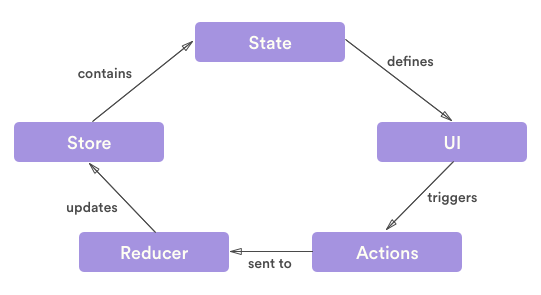
\includegraphics[width=14cm]{react_workflow}}
\caption{ Workflow of react application }
\label{fig:react_workflow}
\end{figure}

\clearpage
\subsection{Sprint 4}
In this sprint we mostly focused on the authentication and the authorization part
of the application.
\subsubsection{Authentication}
To authenticate users we used Google+ API. Since all developers in Predictix
have @predictix.com Google account they can use it to authenticate to the
application check \hyperref[fig:perf-runner-log]{\ref{fig:perf-runner-log}}. If
it's first login, a new user will be stored in the database. Then all future
requests will be associated to that user using JWT token. The figure
\hyperref[fig:perf-runner-log]{\ref{fig:perf-runner-log}} shows the list of the
account that the user should select from after he click Login with Google
button.

\begin{figure}[h]
  \centerline{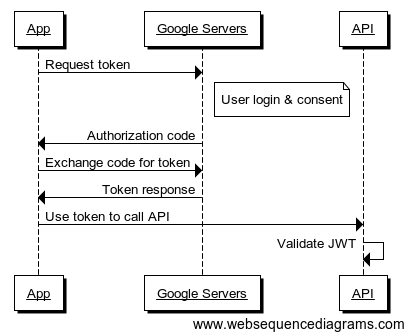
\includegraphics[width=14cm]{google_auth}}
\caption{Google authentication workflow}
\label{fig:google_auth}
\end{figure}

\begin{figure}[h]
  \centerline{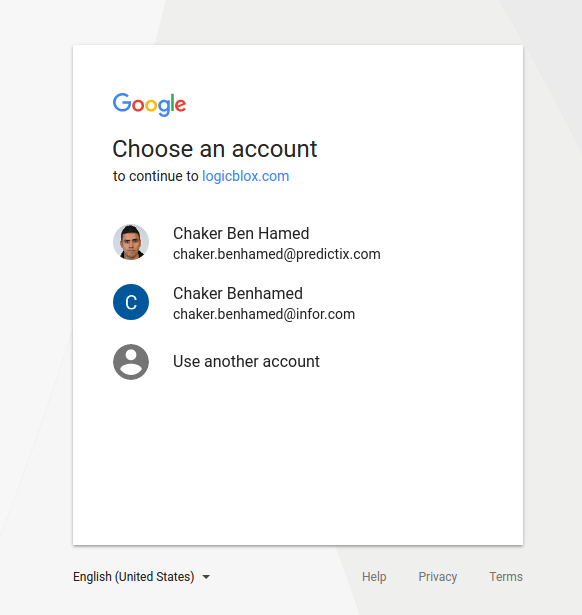
\includegraphics[width=8cm]{chose_google_account}}
\caption{User's Google accounts}
\label{fig:google_auth}
\end{figure}

\subsubsection{Authorization}
Since the application is used to check the performance of Predictix application.
Project owner choose to allow all application user the right to check all
accounts benchmarks and history. However, for running new benchmarks the user
must have the appropriate rights. Thus, we associated an account role to every
user. So either the user have a create benchmark right, admin right or it have
only read right. Check the entity relationship diagram
\hyperref[fig:user_role]{\ref{fig:user_role}} that explain how this is
done in the database
\begin{figure}[h]
  \centerline{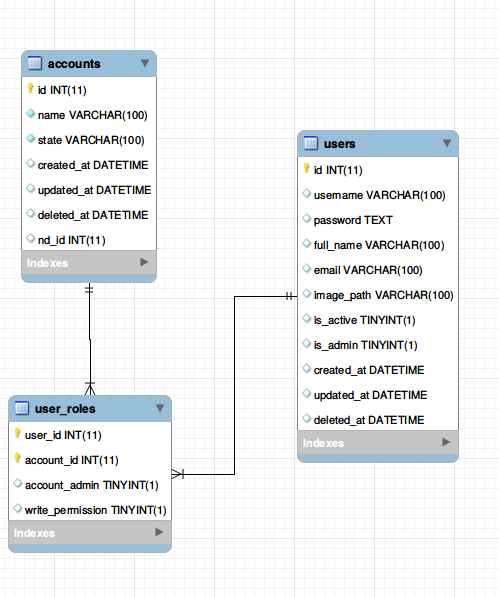
\includegraphics[width=9cm]{user_role}}
\caption{User Role entity}
\label{fig:user_role}
\end{figure}
We use the entity in every user request to check if the user has the appropriate
right, If not we use Pyramid exceptions to return the 403 HTTP response to the
user.

\subsubsection{Security}
Application performance is confidential internal information that shouldn't be
shared out of the company . Thus the application that serve the result should
only be accessible to company employees only. For that we used EC2 security
groups.
EC2 security group \cite{ec2_sg} are network rules that can be set on Amazon cloud instances.
So the application will only be accessibly from certain IPs. We only allowed
access to people who are connected to the company internal VPN.

On top of that we setup an HTTPS certificate and we redirect all non-secured
request to use the HTTPS protocol on port 443. The
figure\hyperref[fig:https]{\ref{fig:https}} show How Google Chrome is
confirming that the site is using a valid HTTPS certificate.
\begin{figure}[h]
  \centerline{
\includegraphics[width=9cm]{https}}
\caption{The HTTPS certificate view in Chrome}
\label{fig:https}
\end{figure}

\section{Final overview}
In this section we will list the final state of the development of the
application. Figure \hyperref[fig:entity_relation]{\ref{fig:entity_relation}} present the
entity-relationship diagram we established by the end of sprint 4. The diagram
show the different entities of the application. Figure
\hyperref[fig:api_doc]{\ref{fig:api_doc}} on the other hand
shows the endpoints of the application API and the documentation of each one,
this include the parameters, URL, payload and the expected result.

\begin{figure}[h]
  \centerline{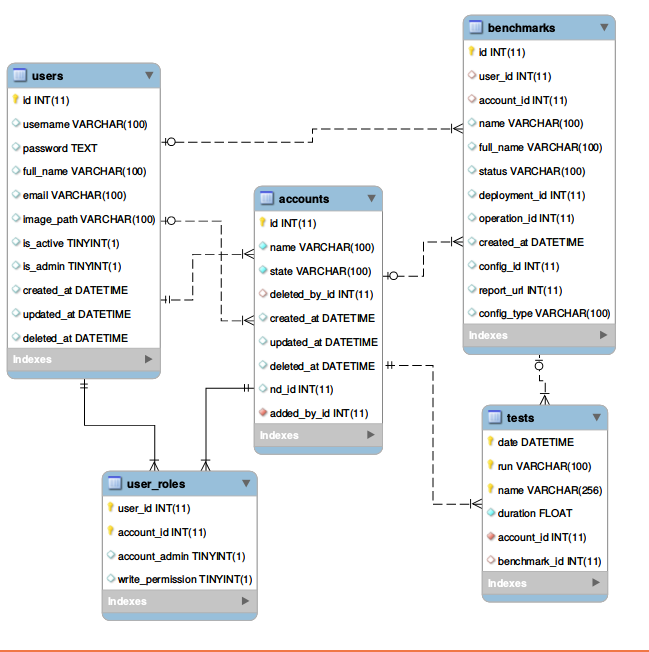
\includegraphics[width=9cm]{entity_relation}}
\caption{Entity relationship diagram}
\label{fig:entity_relation}
\end{figure}

\begin{figure}[h]
  \centerline{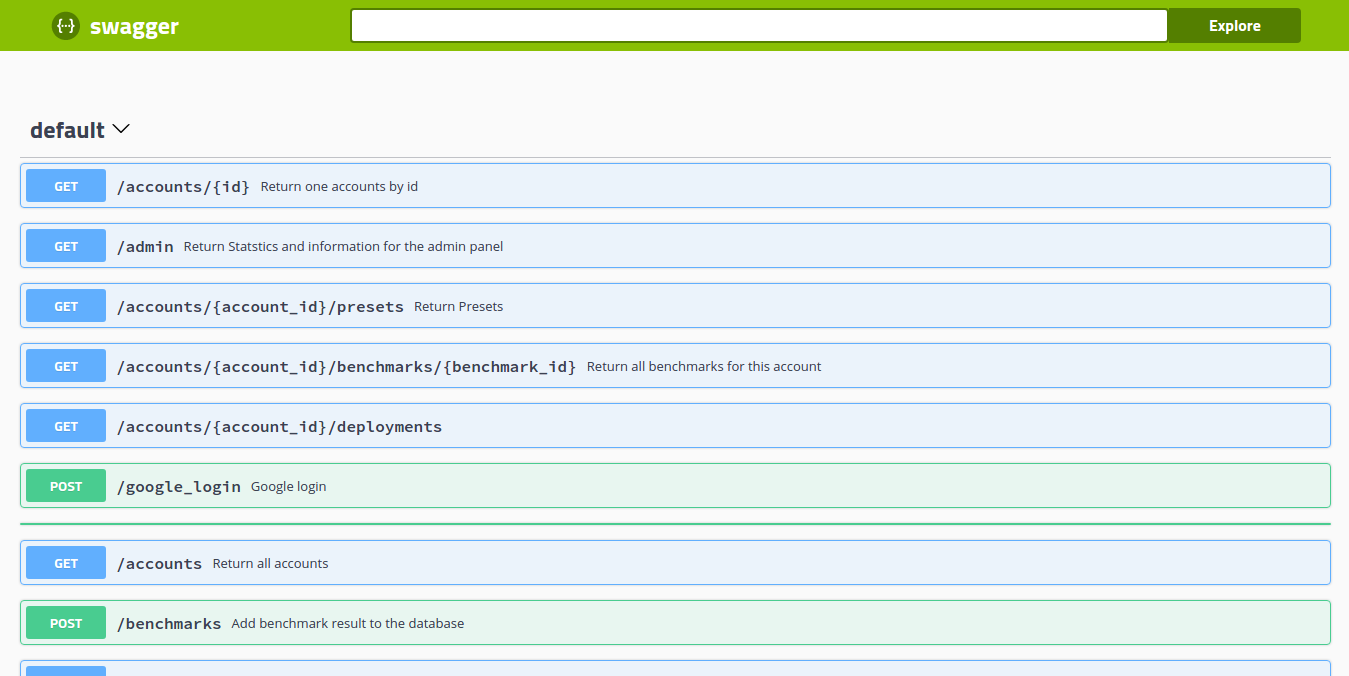
\includegraphics[width=9cm]{api_doc}}
\caption{API documentation}
\label{fig:api_doc}
\end{figure}


\section{Validation tests and Deployment}
Hydra is a Nix-based continuous build system that constantly checks out code
sources of software projects from version management systems such as Mercurial,
to build, test and release them. The build tasks are described using Nix
expressions. This allows a Hydra build task to specify all the dependencies
needed to build or test a project.

In fact, the code of our application is, currently and constantly pushed in a
repository in BitBucket, which is a web-based hosting service for projects that
use either the Mercurial or Git revision control systems, such as GitHub. In
order to have our application ready to be deployed, we added a file called
default.nix to our project, that actually defines the project's nix-expressions.
Afterwards, we created a project under Hydra, that we called \emph{Benchmarks
  Dashboard}. Thus, the \emph{Benchmarks Dashboard} project on Hydra, will be
pulling our code from our BitBucket repository along with the default.nix file
in order to perform the automated build and unit-tests.

The following are some screen shots about our Hydra project build. The figure
\hyperref[fig:hydra_configuration]{\ref{fig:hydra_configuration}}
represents the configuration for our project. We can notice that the links to the
different project's dependencies are defined, such as our source code and the
nixpkgs repository which contains the definitions for all packages available through
the nix package manager.

\begin{figure}[h]
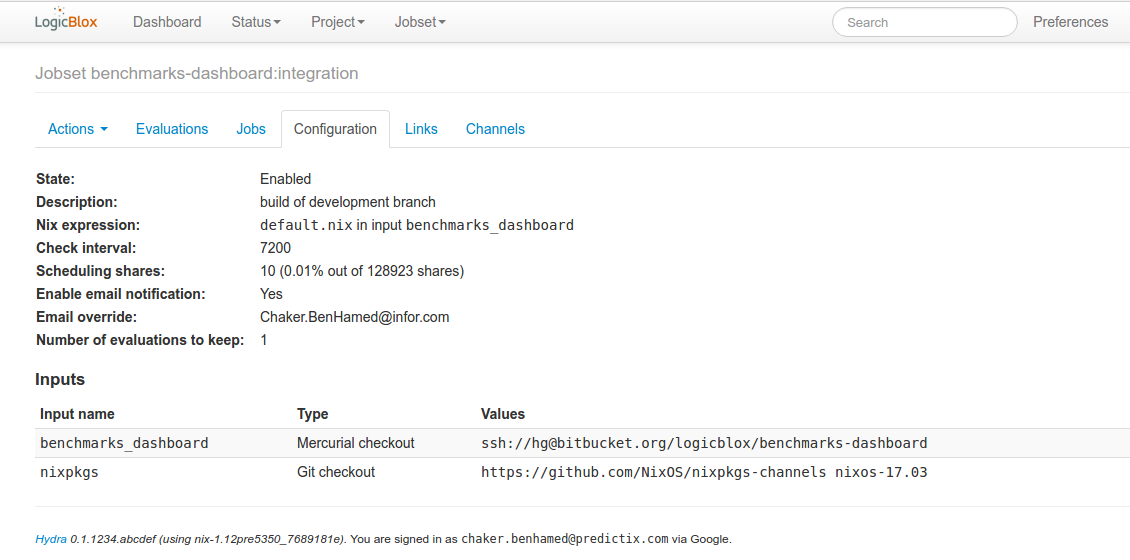
\includegraphics[width=17cm]{hydra_configuration}
\caption{Benchmarks Dashboard Hydra configuration screen}
\label{fig:hydra_configuration}
\end{figure}

The figure \hyperref[fig:hydra_eval]{\ref{fig:hydra_eval}} represents the Hydra
evaluation screen, where we can see the history if the build and whether there
are errors in the build or not.

\begin{figure}[h]
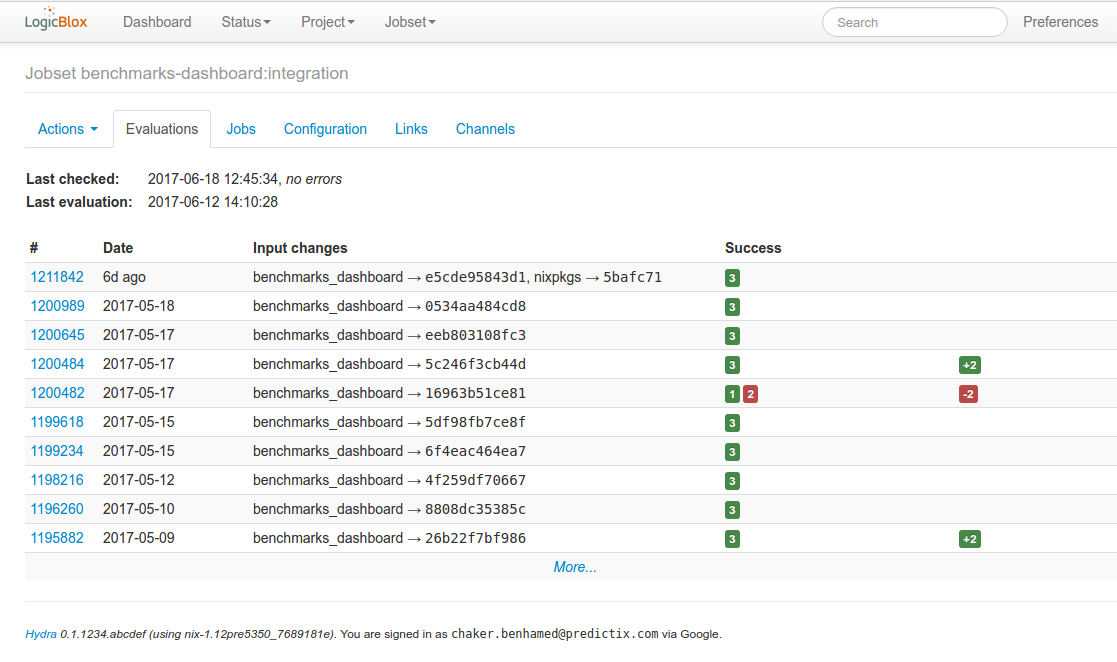
\includegraphics[width=17cm]{hydra_eval}
\caption{Benchmarks Dashboard Hydra evaluations}
\label{fig:hydra_eval}
\end{figure}

In Hydra we can also run unit test and report various indicator about the
quality of the application. The figure
\hyperref[fig:coverage]{\ref{fig:coverage}} shows the coverage report of the test
of our application.

\begin{figure}[h]
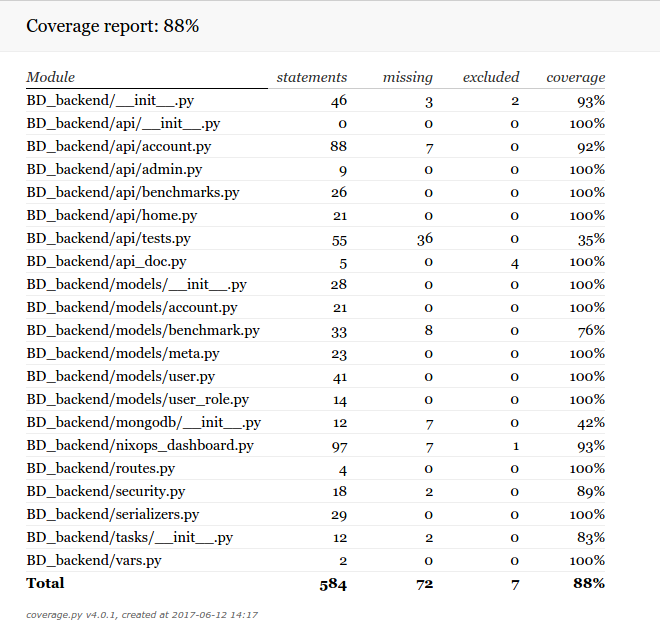
\includegraphics[width=17cm]{coverage}
\caption{Coverage report}
\label{fig:coverage}
\end{figure}

\clearpage
\section*{Conclusion}
For developing the Benchmarks Dashboard, we opted for the scrum methodology
based on incremental development. This section was devoted to the definition of
the sprints we fixed as well as the hardware and software technologies that we
used. We, also, presented the results of the execution of the application
through its interfaces, and our application's deployment process, while giving
the performance evaluation.

\chapter*{General conclusion}

Big data and Cloud computing is the latest buzzwords in information technology.
Having tremendous amounts of complex data that need to be proceed on near
real-time performance, can be tricky. So having a clear performance audit is
critical to monitor the performance of the application. Also providing the way
to the developer to start new benchmark in a click of a button is a major
productivity boost.

In the present report, we began by presenting the general context of our
project while introducing some important concepts, such as deploying,
Benchamrks, workflows and Nix that is used across all of Predictix projects’ and that
we used, as a consequence. We also stated our project’s problematic and an
overview over its goals. Then, we defined our project’s requirements and we
specified them, following the scrum methodology. Afterwards, we proceeded with
the project design through mockups, while defining our project’s static and
behavioural aspect. Finally, we described in the last chapter the
implementation, performance evaluation and deployment processes and presented an
overview of the achieved work.

My internship at Predictix was, undoubtedly, one of the most important and
enriching experiences in my life. This experience was rewarding for me in
terms of academic achievements and professional experience. Indeed, my
internship assignment allowed me to put my academic knowledge into practice
and to gain experience in software development. This was accomplished through
successfully completing development tasks. But added to these technical
competencies, I have also acquired soft skills through the daily experience of
working within the team of developers at Predictix as we had the opportunity to
work in an encouraging, collaborating and teamwork driven environment of
highly skilled engineers.
